\documentclass{article}

\usepackage{microtype}
\usepackage{amsmath}
\usepackage{enumitem}
\usepackage{etoolbox}
% \usepackage{pgfplots}
\usepackage[svgnames]{xcolor}
\usepackage{tikz}
\usepackage[letterpaper]{geometry}

% \pgfplotsset{compat=1.18}

\newcommand{\diff}[1]{\frac{#1}{dt}}
\newcommand{\vel}{\mathrm{v}}
\newcommand{\x}{\mathrm{x}}
\newcommand{\inter}{\int_{t_1}^{t_2}}
\newcommand{\tvert}{\biggr\rvert_{t_1}^{t_2}}
\newcommand{\derv}{\frac{\mathrm{d}}{\mathrm{d}t}}

\patchcmd\subequations
 {\theparentequation\alph{equation}}
 {\subequationsformat}
 {}{}

\newcommand{\subequationsformat}{\theparentequation.\arabic{equation}}

\author{Laith}
\title{Introduction to Physics}
\date{1/25/2023}

\begin{document}
	\maketitle
	\section{What is Physics?}
	Physics is the study of how the objects around us change over time. 
	This includes their \textbf{position}, \textbf{displacement}, \textbf{distance}, and \textbf{speed}.
	\subsection{Position}
	The \textbf{position} of an object is its relative distance from a reference point. For example, if we had a red dot and a green dot on a line, then we could
	determine the position of the red dot to be its distance from the green dot and the position of the green dot to be its distance from the red dot.
	We can express position as a function $\mathrm{x(t)}$.
	\subsection{Displacement}
	\textbf{Displacement} is the difference between an objects new position and its previous position. If we had a red dot move from point 1 to point 2, then the
	displacement of the red dot would be the difference in position of point 2 and point 1.
	Mathematically, we can represent this as $\Delta{x}$.
	\[\Delta{x} = x_2-x_1\]
	Since position is a function, $x_2$ and $x_1$ can be written as $x(t_2)$ and $x(t_1)$, where $t_2$ is the time at which
	the object was at position 2 and $t-1$ is the time at which the object was at position 1. Thus, we can write 
	displacement as:
	\[\Delta{x} = \mathrm{x(t_2)}-\mathrm{x(t_1)}\]  
	\subsection{Distance}
	\textbf{Distance} is the length of the path traveled by an object from one point to another.
	\subsection{Speed}
	\textbf{Speed} is how fast an object moved from one point to another. As an extension, \textbf{velocity} is just speed, but in specific direction. In other words,
	speed is a \emph{scalar}, velocity is a \emph{vector}, but both represent how fast an object moves. The rate at which velocity change over time is known as \textbf{acceleration}.
	We can represent velocity as a function $\mathrm{v(t)}$. We could try to define this function as the ratio between displacement and time elapsed between two points:
	\[\overline{\mathrm{v(t)}} = \frac{\Delta{x}}{\Delta{t}}\]
	The issue with this equation is that velocity can change at any given time, thus in order to get closer to a true representation
	of velocity, we need to look at instantaneous intervals of velocity. In other words: we differentiate position.
	\[\mathrm{v(t)} = \diff{dx}\]
	By differentiating position, we will get the rate at which position changes at a specific time $t$, which is the velocity at that specific time.
	\subsection{Acceleration}
	\textbf{Acceleration} is the rate at which the velocity of an object changes, however with a few exceptions,
	we will assume acceleration to be constant for the majority of this course. Thus, we will represent
	acceleration as a variable $a$, and if acceleration is not constant, a function $\mathrm{a(t)}$.

	Since acceleration is the rate at velocity changes, we can differentiate velocity to get acceleration:
	\[\mathrm{a} = \diff{dv}\]
	This also means that if we want to get velocity, but only have acceleration, we can integrate acceleration to get
	velocity:
	\begin{align*}
	\mathrm{v(t)\biggr\rvert_{t_1}^{t_2}} & = \int_{t_2}^{t_1}a\,dt\\
	\mathrm{v(t)\biggr\rvert_{t_1}^{t_2}} & = a\cdot t\biggr\rvert_{t_1}^{t_2}\\
	\mathrm{v(t)\biggr\rvert_{t_1}^{t_2}} & = a\cdot t_2 - a \cdot t_1 = a\cdot (t_2-t_1)\\
	\mathrm{v(t_2)-v(t_1)} & = a\cdot(t_2 - t_1)
	\end{align*}
	\section{Time}
	Objects always move with respect to time, as the definition of physics would imply. Thus, we treat time as an independant variable; while position, displacement,
	distance, speed, velocity, and acceleration are all functions of time.
	\section{Problems}
	\subsection{The Rabbit}
	A rabbit is moving along a straigh line. At time $t_1=0$ the raddit is distance $x_1=1\mathrm{m}$ from your right
	and is moving towards the right with a velocity of $v_1=1\mathrm{\frac{m}{s}}$. The rabbit has a constant acceleration
	of $a=1\mathrm{\frac{m}{s^2}}$ towards the right. What is the position of the rabbit as time $t_2=10s$?
	\subsubsection{Solution}
	First we list our known variables followed by our unknowns:
	\begin{align*}
	&\mathrm{\underline{Knowns}}\\
	&x_1 =1\mathrm{m} \\
	&t_1 =0\mathrm{s}\\
	&v_1 =1\mathrm{\frac{m}{s}} \\
	&t_2 = 10\mathrm{s}\\
	&a =1\mathrm{\frac{m}{s^2}}\\
	&\mathrm{\underline{Unknowns}}\\
	&x_2 = ?\\
	&v_2 = ?
	\end{align*}
	Then we illustrate the scenario:
	\begin{figure}[hh]
	\begin{center}
	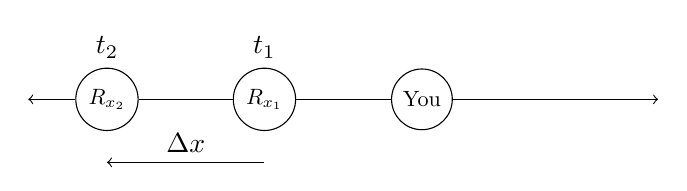
\begin{tikzpicture}
		\node[above] at (3, 0.4) (t1) {$t_1$};
		\node[above] at (1, 0.4) (t2) {$t_2$};
		\node[circle, draw, scale=0.8] at (3, 0) (r) {$R_{x_1}$};
		\node[circle, draw, scale=0.8] at (1, 0) (r2) {$R_{x_2}$};
		\node[circle, draw, scale=0.8] at (5, 0) (y) {You};

		\draw[<-] (0, 0) -- (r2);
		\draw (r2) -- (r);
		\draw (r) -- (y);
		\draw[->] (y) -- (8, 0);

		\node[above] at (2, -0.8) (x) {$\Delta{x}$};

		\draw[<-] (1, -0.8) -- (3, -0.8);
	\end{tikzpicture}
	\end{center}
    \end{figure}
	% \newpage
	While we do know velocity at time $t=0\mathrm{s}$, we do not know velocity at time $t=10\mathrm{s}$.
	We don't need to know the value of velocity at this point, it will give us the grounds to define an expression
	for $\mathrm{v(t)}$, which we can differentiate to get a function for position, allowing us to calculate the final
	position of the rabbit.

	Since we know acceleration $a=1\mathrm{\frac{m}{s^2}}$, including the fact that it is constant, we can
	differentiate acceleration to find a function for velocity:
	\begin{subequations}
	\begin{align}
		a &= \diff{dv}\\
		\int_{t_2}^{t_1}a\,dt &= \int_{t_2}^{t_1}\diff{dv}\\
		a\cdot t\biggr\rvert_{t_1}^{t_2} &= \mathrm{v}(t) \biggr\rvert_{t_1}^{t_2}\\
		&\Rightarrow \mathrm{v}(t_2)-\mathrm{v}(t_1) = a\cdot(t_2 - t_1)\\
		&\Rightarrow \mathrm{v}(t_2) = a\cdot (t_2-t_1) + \mathrm{v}(t_1)
	\end{align}
	Now that we have a function for velocity, we can utilize the fact that velocity
	is the derivative of position, allowing us to set our function equal to $dx$:
	\[\diff{dx} = \mathrm{v}(t_2) = a\cdot(t_2-t_1)+\mathrm{v}(t_1)\]
	We can now omit $\mathrm{v}(t_2)$ since we aren't looking for it, giving us a clean equation that we
	can integrate to get the value of $x_2$. Naturally, we want to integrate with the upper limit 
	$t_2$ and the lower limit $t_1$:
	\begin{align}
		\int_{t_1}^{t_2} \diff{dx}\,dt &= \int_{t_1}^{t_2} [a\cdot (t_2-t_1) + v_1] \,dt\\
		\int_{t_1}^{t_2}\diff{dx}\,dt &= \int_{t_1}^{t_2} a\cdot(t_2-t_1)\,dt + \int_{t_1}^{t_2} v_1\,dt\\
		\mathrm{x}(t)\biggr\rvert_{t_1}^{t_2} &= \int_{t_1}^{t_2}(a\cdot \Delta{t}) \,dt + (v_1\cdot t) \biggr\rvert_{t_1}^{t_2}\\
		\mathrm{x}(t)\biggr\rvert_{t_1}^{t_2} &= a\frac{\Delta{t}^2}{2} \biggr\rvert_{t_1}^{t_2} + (v_1\cdot t) \biggr\rvert_{t_1}^{t_2}
	\end{align}
	Note: $\Delta{t} = t - t_1$ where $t$ is a parameter.
	\begin{align}
		\mathrm{x}(t_2)-\mathrm{x}(t_1) &= a(\frac{\Delta{t}^2(t_2)}{2} - \frac{\Delta{t}^2(t_1)}{2}) + v_1\cdot (t_2-t_1)\\
		\mathrm{x}(t_2)-\mathrm{x}(t_1) &= a(\frac{(t_2-t_1)^2}{2} - \frac{(t_1-t_1)^2}{2}) + v_1\cdot (t_2-t_1)\\
		\mathrm{x}(t_2) &= a(\frac{(t_2-t_1)^2}{2} - \frac{(t_1-t_1)^2}{2}) + v_1\cdot (t_2-t_1) + \mathrm{x}(t_1)\\
		x_2 &= a(\frac{(t_2-t_1)^2}{2} - \frac{(t_1-t_1)^2}{2}) + v_1\cdot (t_2-t_1) + x_1\\
	\end{align}
	We now have an equation for $x_2$. Now all we need to do now is plug in our knowns.
	\begin{align}
		x_2 &= (1)(\frac{(10-0)^2}{2} - \frac{(0-0)^2}{2}) + (1)\cdot (10-0) + (1)\\
		x_2 &= 1(\frac{(10)^2}{2} - \frac{(0)^2}{2}) + 1\cdot 10 + 1\\
		x_2 &= 1(\frac{100}{2} - \frac{0}{2}) + 10 + 1\\
		x_2 &= 1(50 - 0) + 11\\
		x_2 &= 50 + 11\\
		x_2 &= 61\\
	\end{align}
	\end{subequations}
	Our answer: $61\mathrm{m}$. The final position of the rabbit (the position of the rabit at
	time $t_2=10\mathrm{s}$) is $61$ meters from our right.
	\subsection{The Police Car and the Speeding Car}
	A car is moving with a constant speed $v$. It passes a police car on the side of the road.
	The officer realized that the speed of the car was over the limit and starts to chase it at
	time $t_1=10\,\mathrm{s}$ after the car passed by. The police car moves with a constant acceleration 
	of $a=10\,\mathrm{m/s^2}$ and reaches the car at $t_2=30\,\mathrm{s}$. What is the velocity of the
	speeding car?
	\subsubsection{Solution}
	Lets draw the scenario:
	\begin{figure}[hh]
	\begin{center}
	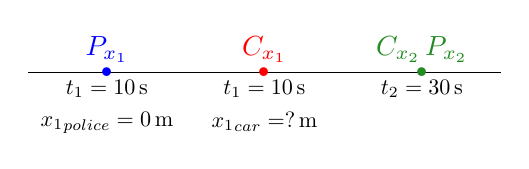
\begin{tikzpicture}
		\draw[] (-1, 0) -- (5, 0);

		\node[above, scale=1, color=blue] at (0, 0) (p) {$P_{x_1}$};
		\node[above, scale=1, color=red] at (2, 0) (c) {$C_{x_1}$};
		\node[above, scale=1, color=ForestGreen] at (4, 0) (x) {$C_{x_2}\,P_{x_2}$};

		\node[scale=3, color=blue] at (0, 0) (p1) {.};
		\node[scale=3, color=red] at (2, 0) (p2) {.};
		\node[scale=3, color=ForestGreen] at (4, 0) (p3) {.};
		
		\node[below, scale=0.8] at (0, 0) (p) {$t_1=10\,\mathrm{s}$};
		\node[below, scale=0.8] at (2, 0) (c) {$t_1=10\,\mathrm{s}$};
		\node[below, scale=0.8] at (2, -0.4) (x) {${x_1}_{car}=?\,\mathrm{m}$};
		\node[below, scale=0.8] at (4, 0) (x) {$t_2=30\,\mathrm{s}$};
		\node[below, scale=0.8] at (0, -0.4) (x) {${x_1}_{police}=0\,\mathrm{m}$};
	\end{tikzpicture}
	\end{center}
    \end{figure}

	Lets list our known and unknown variables:
	\begin{align*}
		&\mathrm{\underline{Knowns}}\\
		&t_1 =10\,\mathrm{s} \\
		&t_2 = 30\,\mathrm{s} \\
		&{v_1}_{police} =0\,\mathrm{m/s} \\
		&a_{police} =10\,\mathrm{m/s^2}\\
		&{x_1}_{police} = 0\,\mathrm{m}\\
		&a_{car} =0\,\mathrm{m/s^2}\\
		&\mathrm{\underline{Unknowns}}\\
		&{x_1}_{car} = ?\\
		&x_2 = ?\\
		&{v_2}_{police} = ?\\
		&{v}_{car} = ?
	\end{align*}
	We will make the initial position of the police car our reference position, thus it will
	be equal to $0\,\mathrm{m}$. Since the speeding car has a constant speed, its acceleration
	equals $0\,\mathrm{m/s^2}$ because the speed is not changing. 

	We can prove this mathematically via the fact that taking the derivative of a constant will 
	return $0$, and since acceleration is the derivative of velocity, our acceleration would be $0$.

	In order to find the velocity of the speeding car, we need to consider the fact that the police car 
	eventually reaches the speeding car, in which the police car started at a velocity of $0\,\mathrm{m/s}$
	at time $t_1=10\,\mathrm{s}$ and reaches the speeding car at an unknown velocity at time $t_2=30\,\mathrm{s}$.
	In order to reach the speeding car, the police car would have to reach a speed higher than the speeding car, thus
	at some time $t$, $\vel_{police}(t) = \vel_{car}(t)$, and since the velocity of the speeding car is constant,
	$\vel_{police}(t) = v_{car}$. In order to find the velocity of the speeding car, we need to find the time at which 
	the two velocities were equal. 
	\begin{subequations}
	\begin{align}
		\vel_{police}(t) &= v_{car}
	\end{align}
	We can integrate the acceleration of the police car to get $\vel(t)$. 
	\begin{align}
		\vel_{police}(t) &= \int a_{police} \,dt \\
		\vel_{police}(t) &= \int 10 \,dt \\
		\vel_{police}(t) &= 10t + C
	\end{align}
	In order to get rid of the unknown constant $C$, we can set our limits to be $b=t$ where $t$ is the time 
	we are looking for and $a=t_1$ where $t_1=10\,\mathrm{s}$. 
	\begin{align}
		\vel_{police}(t) \biggr\rvert_{t_1}^{t} &= 10t + C \biggr\rvert_{t_1}^{t} \\
		\vel_{police}(t) \biggr\rvert_{10}^{t} &= 10t + C \biggr\rvert_{10}^{t} \\
		\vel_{police}(t) - \vel_{police}(10) &= [10(t) + C] - [10(10) + C] \\
		\vel_{police}(t) - \vel_{police}(10) &= 10(t) - 10(10) \\
		\vel_{police}(t) - \vel_{police}(10) &= 10t - 100
	\end{align}
	Since we know that the police car only starts to move at time $t_1=10\,\mathrm{s}$, we know that
	$\vel_{police}(10) = 0$.
	\begin{align}
		\vel_{police}(t) - (0) &= 10t - 100 \\
		\vel_{police}(t) &= 10t - 100
	\end{align}
	What this gives us is a function that tells the velocity of the police car for time $t \geq 10$.

	Now, $v_{police}(t) = v_{car}$ if $30 > t > 10$. Since both cars reach the same position at time $t_2=30\,\mathrm{s}$,
	we can integrate velocity with limits $b=t$ and $a=t_1=10\,\mathrm{s}$ to get position, and then calculate the position at
	time $t=30\,\mathrm{s}$. 
	\begin{align}
		\x_{police}(t) \biggr\rvert_{t_1}^{t} &= \int_{t_1}^{t} \vel_{police}(t) \,dt \\
		\x_{police}(t) \biggr\rvert_{t_1}^{t} &= \int_{t_1}^{t} 10t - 100 \,dt \\
		\x_{police}(t) \biggr\rvert_{10}^{t} &= \int_{10}^{t} 10t - 100 \,dt \\
		\x_{police}(t) - \x_{police}(10) &= [10\frac{t^2}{2} - 100t] \biggr\rvert_{10}^{t} \\
		\x_{police}(t) - \x_{police}(10) &= [5t^2 - 100t] \biggr\rvert_{10}^{t} \\
		\x_{police}(t) - \x_{police}(10) &= [5t^2 - 100t] - [5(10)^2 - 100(10)] \\
		\x_{police}(t) - \x_{police}(10) &= [5t^2 - 100t] - (-500) \\
		\x_{police}(t) - \x_{police}(10) &= 5t^2 - 100t + 500 \\
	\end{align}
	Since we decided that the initial position of the police car would be our reference point, we know that
	$\x_{police}(10)=0$.
	\begin{align}
		\x_{police}(t) - (0) &= 5t^2 - 100t + 500 \\
		\x_{police}(t) &= 5t^2 - 100t + 500
	\end{align}	
	If $\x_{police}(t) = \x_{car}(t)$ at time $t=30\,\mathrm{s}$, we can integrate the velocity of the speeding car $v_{car}=C$
	with the limts $b=t$ and $a=t_1=10\,\mathrm{s}$ to get its position function $\x_{car}(t)$. 
	Then, we can set the position functions of both cars equal to each other, allowing us to solve for $C$.
	\begin{align}
		\x_{car}(t)  &= \int_{t_1}^{t} v_{car} \,\mathrm{d}t \\
		\x_{car}(t)  &= \int_{t_1}^{t} C \,\mathrm{d}t \\
		\x_{car}(t)  &= C\cdot t \biggr\rvert_{t_1}^{t} \\
		\x_{car}(t) &= C\cdot t \biggr\rvert_{10}^{t} \\
		\x_{car}(t)  &= C\cdot t - C\cdot 10 \\
		\x_{car}(t)  &= C\cdot (t - 10) \\
	\end{align}
	Now we set the position function of the speeding car equal to the position function of the police car:
	\begin{align}
		\x_{car}(t) \biggr\rvert_{t=30} &= \x_{police}(t) \biggr\rvert_{t=30} \\
		C\cdot(t-10) \biggr\rvert_{t=30} &= 5t^2-100t+500 \biggr\rvert_{t=30} \\
		C\cdot((30)-10) &= 5(30)^2-100(30)+500 \\
		C\cdot(20) &= 5(900)-3000+500 \\
		20C &= 4500-3000+500 \\
		20C &= 1500+500 \\
		20C &= 2000 \\
		\Rightarrow C &= \frac{2000}{20} \\
		C &= 100 \,\mathrm{m/s}
	\end{align}
	\end{subequations}
\end{document}
